%%%%%%%% FlowSNE method paper -- ICML template %%%%%%%%%%%%%%%%%%%%%%%%
% Working draft, started 6 Nov 2026. Replaces the theory-only draft in
% ../ICML (kept as is). Page target: 8 pages of main text.
% Rough budget: intro 1, related work 0.75, background 0.75, Randers
% affinities 2, FlowSNE 1.25, experiments 2 (6.3 reserved), conclusion 0.25.

\documentclass{article}

\usepackage{microtype}
\usepackage{graphicx}
\usepackage{subcaption}
\usepackage{booktabs}
\usepackage{multirow}
\usepackage{hyperref}
\newcommand{\theHalgorithm}{\arabic{algorithm}}

% blind submission; switch to [preprint] or [accepted] as needed
\usepackage{icml2026}

\usepackage{amsmath}
\usepackage{amssymb}
\usepackage{mathtools}
\usepackage{amsthm}
\usepackage[capitalize,noabbrev]{cleveref}

\theoremstyle{plain}
\newtheorem{theorem}{Theorem}[section]
\newtheorem{proposition}[theorem]{Proposition}
\newtheorem{lemma}[theorem]{Lemma}
\newtheorem{corollary}[theorem]{Corollary}
\theoremstyle{definition}
\newtheorem{definition}[theorem]{Definition}
\theoremstyle{remark}
\newtheorem{remark}[theorem]{Remark}

\usepackage[textsize=tiny]{todonotes}
\newcommand{\tbd}[1]{\textcolor{red}{[TODO\ifx\relax#1\relax\else: #1\fi]}}

% ---------------------------------------------------------------- macros
\newcommand{\R}{\mathbb{R}}
\newcommand{\eps}{\varepsilon}
\newcommand{\1}{\mathbf{1}}
\newcommand{\diag}{\operatorname{diag}}
\newcommand{\Sep}{\mathcal{S}}
\newcommand{\Asym}{\mathcal{A}}
\newcommand{\Grad}{\mathcal{G}}
\newcommand{\cyc}{\operatorname{cyc}}
\newcommand{\Sk}{\operatorname{Sk}}
\newcommand{\RS}{\operatorname{RS}}
\newcommand{\dF}{d_F}
\newcommand{\dfr}{\hat d}
\newcommand{\dav}{\bar d}
\newcommand{\E}{\mathbb{E}}

\icmltitlerunning{FlowSNE: Neighbour Embeddings with Randers Costs}

\begin{document}

\twocolumn[
  \icmltitle{FlowSNE: Neighbour Embeddings of Data with Velocities\\
    through Randers Affinities}

  \begin{icmlauthorlist}
    \icmlauthor{Anonymous}{anon}
  \end{icmlauthorlist}
  \icmlaffiliation{anon}{Anonymous institution}
  \icmlcorrespondingauthor{Anonymous}{anon@anon}
  \icmlkeywords{dimensionality reduction, neighbour embedding, t-SNE, Finsler geometry, Randers metric, optimal transport, Sinkhorn, RNA velocity}
  \vskip 0.3in
]

\printAffiliationsAndNotice{}

\begin{abstract}
  Many datasets come with a direction at each sample: RNA velocity in
  single-cell transcriptomics, the update a transformer layer applies to
  its residual stream, the velocity of a generative flow. Neighbour
  embeddings such as t-SNE build their affinities from a symmetric cost,
  so they discard this direction, and velocities are usually projected
  onto the layout afterwards. We introduce FlowSNE, a neighbour
  embedding in which both the input affinity and the embedding kernel are
  built from a \emph{Randers} cost, the simplest direction-dependent
  (Finsler) metric: moving with the drift is cheaper than moving against
  it. On the input side, closed-form approximations of the Randers
  distance, with explicit error bounds, turn per-sample velocities into an
  entropic affinity. We show that its normalisation decides what it
  encodes: a Sinkhorn-balanced affinity sees the drift only modulo
  gradients, keeping its circulation and discarding its potential part,
  while a row-stochastic one keeps both. On the output side, a small
  neural network fits a drift field in the embedding jointly with the
  layout, so that the layout and its arrows come from the same model.
  A KeOps implementation in TorchDR scales to $10^5$ points on one GPU.
  On synthetic flows and on single-cell datasets up to
  \tbd{N}~cells, FlowSNE gives better layouts and speed estimates than
  spectral Finsler embeddings at comparable direction accuracy, and its
  own directed kernel keeps the developmental progression that
  symmetric embeddings lose.
  \todo[inline]{Abstract to be revised once Sections 6.2, 6.3 and 7 exist.}
\end{abstract}


% ======================================================================
\section{Introduction}
\label{sec:intro}

\begin{figure}[t]
  \centering
  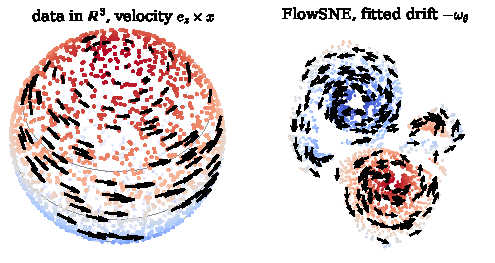
\includegraphics[width=\columnwidth]{figures/teaser_sphere.pdf}
  \caption{\emph{Left:} points on a sphere with a rotation velocity
  $e_z\times x$, coloured by height (red north, blue south).
  \emph{Right:} the 2-D FlowSNE embedding (row-stochastic input), fitted
  jointly with a drift field (arrows), same colours. The map tears the
  sphere along the equator; each hemisphere becomes a vortex centred on the
  image of its pole, where the true speed vanishes.}
  \label{fig:teaser}
\end{figure}

Neighbour embeddings are the standard way to look at high-dimensional
data. SNE, t-SNE and UMAP
\citep{hinton2002sne,vandermaaten2008tsne,mcinnes2018umap} turn pairwise
costs into an affinity matrix and fit a low-dimensional layout whose own
affinities match it. Their costs are symmetric: the affinity of $x_j$
seen from $x_i$ is built from the same number as that of $x_i$ seen
from $x_j$.

Many datasets, however, come with a \emph{direction} at each sample. In
single-cell transcriptomics, \emph{RNA velocity} estimates, for every
cell, where its gene expression is heading in the next hours
\citep{lamanno2018rna,bergen2020generalizing}: each data point comes with
a velocity vector in the same space. In a transformer, each layer adds an
update to the residual stream of every token. A flow-matching model
carries a velocity field by construction. A symmetric cost cannot express
that moving \emph{with} such a field is easier than moving against it,
so neighbour embeddings discard the direction. The common workaround
draws arrows afterwards. scVelo \citep{bergen2020generalizing}, the
standard tool in single-cell analysis, first fits a symmetric embedding,
then for each cell compares its velocity with the directions to its
neighbours in the data space, and draws an arrow towards the neighbours
the velocity points to, at their positions in the layout. The arrow
depends on the layout and on its neighbourhood graph, can only point
towards neighbours the symmetric map placed nearby, and may show a
direction the data do not support \citep{bergen2021rna}. The direction
is painted onto the map; it did not shape it.

The simplest direction-dependent geometry is a \emph{Randers} metric
\citep{randers1941asymmetrical,bao2000introduction}, a Euclidean norm
tilted by a drift field $\omega$ with $\|\omega\|<1$:
\begin{equation}
  F_x(v)=\|v\|+\omega(x)^\top v .
  \label{eq:randers}
\end{equation}
Moving along $\omega$ costs $1+\|\omega\|$ per unit length, moving
against it $1-\|\omega\|$. Plugging a Randers distance into the
entropic affinities of SNE seems straightforward, but raises three
questions. The distance is an infimum over paths with no closed form
when $\omega$ varies, so it must be approximated. Affinities are
normalised, by rows (SNE) or by Sinkhorn balancing (SNEkhorn,
\citealt{vanassel2023snekhorn}), and a normalisation rescales rows and
columns, which can absorb part of the asymmetry. Finally, the embedding
kernel must be able to express the direction it is asked to match.

\paragraph{Contributions.}
We introduce \emph{FlowSNE}, a neighbour embedding for data with
velocities (\cref{fig:teaser}), and answer these three questions.
\begin{itemize}
  \item \textbf{Randers affinities (\cref{sec:randers}).} Two closed-form
    approximations of the Randers distance built from the velocities at
    the endpoints only, with error $O(r^2)$ and $O(r^3)$ at distance
    $r$ (\cref{prop:approx}), define a perplexity-calibrated entropic
    affinity.
  \item \textbf{What normalisation keeps (\cref{sec:gauge}).} A
    Sinkhorn-balanced affinity is determined by its cost modulo
    separable functions (\cref{thm:identifiability}). It therefore sees
    the circulation of a drift and not its gradient part, which a
    row-stochastic affinity keeps as a tilt of its column marginal. A
    uniform drift is invisible to a balanced affinity.
  \item \textbf{FlowSNE (\cref{sec:flowsne}).} The embedding kernel is a
    Student kernel on a Randers cost whose drift is a small neural network
    fitted jointly with the layout. The same gauge argument tells which
    part of this drift the loss can reward.
  \item \textbf{Implementation (\cref{sec:implementation}).} A
    TorchDR implementation with KeOps lazy tensors computes both costs
    in $O(n)$ memory and fits $10^5$ points on one GPU.
  \item \textbf{Experiments (\cref{sec:exp}).} On synthetic flows,
    clean or noisy and high-dimensional, FlowSNE recovers circulation,
    which embeddings with a constant Finsler drift cannot represent, and
    matches them in direction on gradient flows. On single-cell data the
    two normalisations behave as the theory predicts: on a
    differentiation process the row-stochastic input keeps the signal,
    while on the cell cycle, where an independent measurement of each
    cell's phase gives a ground truth, the balanced input isolates the
    circulation (0.68 against 0.39 for projected arrows) and the
    row-stochastic one fits the density instead. On GPT-2's residual
    stream, FlowSNE orients the rings that calendar tokens form.
\end{itemize}


% ======================================================================
\section{Related work}
\label{sec:related}

\paragraph{Dimensionality reduction.}
Linear methods, PCA \citep{pearson1901pca} and classical MDS
\citep{torgerson1952mds}, preserve variance or pairwise distances.
Manifold learning replaces Euclidean distances by intrinsic ones: graph
geodesics in Isomap \citep{tenenbaum2000global}, local linear
reconstructions in LLE \citep{roweis2000lle}, and the spectrum of a graph
Laplacian in Laplacian eigenmaps \citep{belkin2003laplacian}. Diffusion
maps \citep{coifman2006diffusion} embed with the eigenvectors of a
normalised Markov kernel, so that Euclidean distances in the embedding
approximate diffusion distances; PHATE \citep{moon2019phate} builds on
them for single-cell data. Neighbour embeddings instead match
\emph{affinities}: SNE and t-SNE
\citep{hinton2002sne,vandermaaten2008tsne} calibrate one entropic
bandwidth per point to a target perplexity
\citep{vladymyrov2013entropic} and fit a heavy-tailed kernel in the
embedding; UMAP \citep{mcinnes2018umap} uses fuzzy-set affinities.
SNEkhorn \citep{vanassel2023snekhorn} replaces the row normalisation by
a symmetric entropic optimal-transport problem with controlled marginals,
which removes the hubs and density artefacts of row-stochastic
affinities. All of these build their affinities from symmetric costs, or
symmetrise them before embedding.

\paragraph{Asymmetric data and Finsler embeddings.}
Asymmetric proximities have long been embedded by variants of MDS
\citep{okada1987asymmetric}, and directed graphs by factorising
asymmetric proximity matrices \citep{ou2016hope}. Two recent lines use
Finsler geometry explicitly. Finsler MDS \citep{dages2025finsler}
embeds an asymmetric dissimilarity matrix into a \emph{canonical Randers
space}, Euclidean space with one constant drift, by a Finsler version of
SMACOF; a follow-up \citep{dages2026harnessing} extends t-SNE and UMAP to
that output space. There, the asymmetry comes from the data's sampling
density, through the per-point bandwidths of SNE, and the output drift
is a fixed constant vector: the data carry no velocities, and the
embedding carries no field. \citet{debaussart2026finslerian} start from
directed (e.g.\ Randers) distances and take the diffusion-maps route:
the symmetric part of a $\theta$-normalised directed kernel converges to
a weighted Laplacian, which gives the layout, and its antisymmetric part
to a transport along the centroid field of the Finsler unit ball, which
gives a drift read off that symmetric layout afterwards.

\paragraph{Data with velocities.}
In single-cell biology, RNA velocity
\citep{lamanno2018rna,bergen2020generalizing} is shown by projecting it
onto a precomputed t-SNE or UMAP layout through a transition kernel on
the cells' neighbourhood graph; CellRank \citep{lange2022cellrank} and
dynamo \citep{qiu2022mapping} use such kernels and vector-field
reconstructions to infer fates and dynamics, again on a fixed layout.
None of these lets the velocity shape the layout, and the projected
arrows are known to depend on the embedding \citep{bergen2021rna}.
Velocities also enter optimal-transport costs for learning dynamics from
snapshots: kinematic interpolants \citep{jiang2026kinematic} couple
position--velocity pairs under a cost whose cross term
$(v_i+v_j)^\top(x_j-x_i)$ is, up to scaling, the drift term of our
averaged Randers cost (\cref{sec:randers}). That cost serves to match
two snapshots and fit a second-order dynamics, not to embed one sample.

\paragraph{Position of this work.}
To our knowledge, no neighbour embedding takes per-sample velocities as
input and returns a layout together with a drift field in the
embedding. FlowSNE does so with a Randers cost on both sides; unlike
\citet{dages2026harnessing} the drift varies in space and is learned, and
unlike \citet{debaussart2026finslerian} the layout itself is fitted to
the directed affinity rather than to its symmetric part.


% ======================================================================
\section{Background}
\label{sec:background}

\paragraph{Affinities are normalised kernels.}
Given samples $x_1,\dots,x_n\in\R^D$ and a cost matrix $C$, not
necessarily symmetric, an entropic affinity rescales the rows and columns
of the Gibbs kernel $K_{ij}=e^{-C_{ij}/\eps}$:
\begin{equation}
  P=\diag(\alpha)\,K\,\diag(\beta),\qquad \alpha,\beta\in\R^n_{>0} .
  \label{eq:scaling}
\end{equation}
Normalisations differ in how $\alpha,\beta$ are chosen.
\begin{itemize}
  \item \emph{Row-stochastic} ($\RS$), as in SNE: $\beta=\1$ and
    $\alpha_i=1/(n\,(K\1)_i)$, so that each row is a softmax of
    $-C_{i\cdot}/\eps$ and $P\1=\1/n$.
  \item \emph{Balanced} ($\Sk$): $\alpha,\beta$ solve
    $P\1=P^\top\1=\1/n$ and are found by Sinkhorn iterations
    \citep{sinkhorn1967concerning,cuturi2013sinkhorn}. $\Sk(C)$ is the
    entropic optimal self-transport plan for the cost $C$
    \citep{peyre2019computational}.
\end{itemize}
In practice the bandwidth is calibrated per row, $\eps_i$, so that row
$i$ has a target perplexity
\citep{hinton2002sne,vladymyrov2013entropic}; this divides row $i$ of
$C$ by $\eps_i$. SNEkhorn \citep{vanassel2023snekhorn} adds the
constraint $P=P^\top$, under which $\langle P,C\rangle$ depends only on
$\tfrac12(C+C^\top)$: it discards any asymmetry of the cost by design.

\paragraph{Embedding kernels.}
A neighbour embedding fits $Z=(z_1,\dots,z_n)\in\R^{n\times d}$, $d\ll D$,
by minimising the cross-entropy $-\sum_{ij}P_{ij}\log Q_{ij}(Z)$ between
the input affinity and an embedding kernel. t-SNE uses the Student
kernel
\begin{equation}
  Q_{ij}=\frac{(1+\|z_i-z_j\|^2)^{-1}}{\sum_{k\neq l}(1+\|z_k-z_l\|^2)^{-1}},
  \label{eq:student}
\end{equation}
whose heavy tail lets moderately distant input points spread out in the
embedding \citep{vandermaaten2008tsne}. A symmetric $Q$ only sees
$P+P^\top$: $\sum_{ij}P_{ij}\log Q_{ij}=\tfrac12\sum_{ij}(P_{ij}+P_{ji})\log Q_{ij}$.
Any direction in $P$ is lost unless the embedding kernel is itself
asymmetric.

\paragraph{Randers metrics.}
A Randers norm \eqref{eq:randers} is positive and convex in $v$ if and
only if $\|\omega(x)\|<1$. The Randers distance is the infimum of the
length over paths,
\begin{equation}
  \dF(x\to y)=\inf_{\gamma(0)=x,\ \gamma(1)=y}\int_0^1 F_{\gamma(t)}\big(\dot\gamma(t)\big)\,dt ,
  \label{eq:dF}
\end{equation}
and is asymmetric, $\dF(x\to y)\neq\dF(y\to x)$. Under
\eqref{eq:randers}, moving \emph{along} $\omega$ is \emph{more}
expensive. To make moving with a velocity $v(x)$ cheap, one takes
$\omega=-c\,v$ with $c>0$ small enough for admissibility; the direction
an affinity built on $\omega$ favours is $-\omega$. Constant drifts give
the canonical Randers space of \citet{dages2025finsler}, where
$\dF(x\to y)=\|y-x\|+\omega^\top(y-x)$ exactly.

\paragraph{Plugging a Randers cost into an affinity.}
The natural construction is $C_{ij}=\dF(x_i\to x_j)^q$, with $q=2$ as in
SNE, followed by a normalisation and an embedding. Three questions then
arise, which the next two sections answer. (i) $\dF$ has no closed form
when $\omega$ varies, and $\omega$ is only known at the samples: what
should be computed? (ii) Normalisation rescales rows and columns of a
directed kernel: what part of the drift survives it? (iii) What
embedding kernel can express, and be fitted to, the remaining direction?


% ======================================================================
\section{Entropic Randers affinities}
\label{sec:randers}

\subsection{Randers distances without a closed form}
\label{sec:approx}

The infimum \eqref{eq:dF} has no closed form when $\omega$ varies, and
computing it is impractical for neighbour embeddings, for three reasons
(\cref{app:randers}). Eikonal solvers for asymmetric metrics
\citep{sethian2003ordered,mirebeau2014efficient} need a grid, out of reach
in the $10$ to $50$ dimensions of single-cell data. Graph shortest paths
\citep{tenenbaum2000global} converge only as samples densify along the
optimal paths. Above all, $\omega$ is measured only at the samples,
$\omega_i=\omega(x_i)$, so the infimum over paths through empty regions
depends on an extension of $\omega$ that the data do not determine. We
therefore use costs built from the endpoint values only. With
$\Delta_{ij}=x_j-x_i$,
\begin{align}
  \dfr(x_i\to x_j)&=\|\Delta_{ij}\|+\omega_i^\top\Delta_{ij}
  &&\text{(frozen)},\label{eq:frozen}\\
  \dav(x_i\to x_j)&=\|\Delta_{ij}\|+\tfrac12(\omega_i+\omega_j)^\top\Delta_{ij}
  &&\text{(averaged)}.\label{eq:averaged}
\end{align}
Both are the length of the straight segment from $x_i$ to $x_j$, with the
drift integral replaced by a left-endpoint and a trapezoid rule. The
segment is not a geodesic in general, but it is close to one at short
range, and a kernel only weighs pairs at short range.

\begin{proposition}[Closed-form approximations]
  \label{prop:approx}
  Let $\omega\in C^2(\R^D)$ with $\sup\|\omega\|<1$, and let
  $L_1=\sup\|\nabla\omega\|$, $L_2=\sup\|\nabla^2\omega\|$ and
  $L_c=\sup\|\nabla\omega-\nabla\omega^\top\|$. For $r=\|y-x\|$:
  \begin{enumerate}
    \item $|\dfr(x\to y)-\ell(x,y)|\le\tfrac12L_1r^2$ and
      $|\dav(x\to y)-\ell(x,y)|\le\tfrac1{12}L_2r^3$, where $\ell$ is the
      Randers length of the straight segment;
    \item $0\le\ell(x,y)-\dF(x\to y)\le c\,L_c^2\,r^3$ whenever
      $L_cr\le c'$, for universal constants $c,c'$;
    \item if $\omega=\nabla\phi$, straight lines are geodesics and
      $\dF(x\to y)=\|y-x\|+\phi(y)-\phi(x)$.
  \end{enumerate}
  Hence $\dF-\dfr=O(L_1r^2)$ and $\dF-\dav=O\big((L_2+L_c^2)\,r^3\big)$.
\end{proposition}

Only the curl of $\omega$ makes bending the path worthwhile (item 2), and
for a gradient drift the averaged form is a trapezoid rule for the exact
$\phi(x_j)-\phi(x_i)$. Proofs are in \cref{app:randers}. On gradient
drifts in $D=50$, where $\dF$ is known exactly, the median relative error
over each point's $\sqrt n$ nearest neighbours is $1.5\times10^{-2}$
(frozen) against $1.1\times10^{-4}$ (averaged) for a convex potential,
and $2.3\times10^{-2}$ against $5.7\times10^{-3}$ for a non-convex one.
We use the averaged form throughout; it costs the same. It splits into a
symmetric part $S_{ij}=\|\Delta_{ij}\|$ and an antisymmetric one,
\begin{equation}
  \dav(x_i\to x_j)=S_{ij}+A_{ij},\qquad
  A_{ij}=\tfrac12(\omega_i+\omega_j)^\top\Delta_{ij},
  \label{eq:SA}
\end{equation}
where $A_{ij}=-A_{ji}$ is the work of the drift along the edge, an edge
flow on the complete graph. The frozen form has the same $A$.

\subsection{The affinity}
\label{sec:affinity}

\begin{definition}[Entropic Randers affinity]
  \label{def:era}
  Given samples $x_i$ and velocities $v_i$, let $\omega_i=-\rho\,v_i/\max_k\|v_k\|$
  with $\rho<1$ (default $0.95$), and $C_{ij}=\dav(x_i\to x_j)^q$
  (default $q=2$), $C_{ii}=+\infty$. Calibrate each row's bandwidth $\eps_i$
  by bisection so that the softmax of $-C_{i\cdot}/\eps_i$ has perplexity
  $\mathcal{P}$ (default $\sqrt n$). The \emph{row-stochastic} affinity
  $P^{\RS}$ is that softmax divided by $n$; the \emph{balanced} affinity
  $P^{\Sk}$ rescales the kernel $e^{-C_{ij}/\eps_i}$ to uniform marginals
  by Sinkhorn iterations.
\end{definition}

\begin{figure}[t]
  \centering
  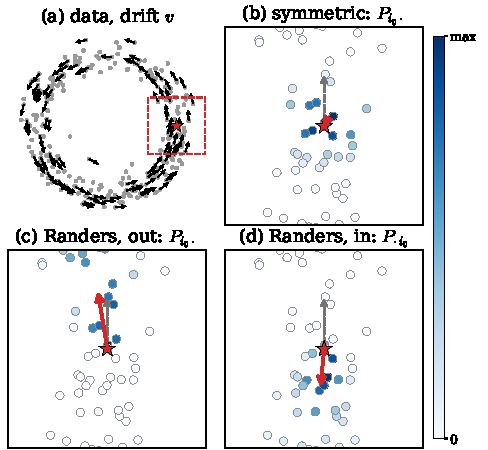
\includegraphics[width=\columnwidth]{figures/randers_affinity.pdf}
  \caption{Neighbourhood of one point $i_0$ ($\star$) on a rotating ring
  ($n=300$, \cref{def:era} with its defaults, balanced). (b--d) zoom on the
  dashed box of (a), one colour scale. Dashed grey: the velocity $v_{i_0}$;
  red: the affinity-weighted mean offset
  $\sum_jP_{ij}(x_j-x_{i_0})/\sum_jP_{ij}$, at true scale. The symmetric
  affinity is direction-blind (offset $0.006$). The Randers affinity sends
  mass downstream (row, offset $0.25$) and receives it from upstream
  (column, $0.17$).}
  \label{fig:randers_affinity}
\end{figure}

\Cref{fig:randers_affinity} shows the effect on a rotating ring: the row
of a point leans downstream, its column upstream. The global rescaling
keeps relative speeds, which a per-point normalisation of $v_i$ would
erase. The perplexity $\sqrt n$ keeps the
neighbourhood a fixed fraction of the data as $n$ grows; we found it
matters at scale (\cref{sec:implementation}). For $\omega=0$,
$P^{\Sk}$ is the balanced entropic affinity of SNEkhorn without the
symmetry constraint, and $P^{\RS}$ is the SNE affinity before
symmetrisation. Which of the two to use is not a detail: they keep
different parts of the drift.

\subsection{What normalisation keeps: a gauge}
\label{sec:gauge}

By \eqref{eq:scaling}, every normalisation adds to $-C/\eps$ a matrix of
the form $f_i+g_j$. Let $\Sep=\{(f_i+g_j)_{ij}:f,g\in\R^n\}$, let $\Asym$
be the antisymmetric matrices and
$\Grad=\{(\psi_j-\psi_i)_{ij}:\psi\in\R^n\}\subset\Asym$ the
\emph{gradient flows}. A short computation (\cref{app:proofs}) gives
$\Sep=\{(s_i+s_j)_{ij}\}\oplus\Grad$ and $\Sep\cap\Asym=\Grad$: the only
antisymmetric costs a rescaling can absorb are differences of a
potential.

\begin{theorem}[Identifiability modulo separable costs]
  \label{thm:identifiability}
  For fixed marginals and a global $\eps$, $\Sk(C)=\Sk(C')$ if and only if
  $C-C'\in\Sep$. In particular, for $C=S+A$ with $S$ symmetric and $A$
  antisymmetric, $\Sk(S+A)=\Sk(S+A')$ if and only if $A-A'\in\Grad$.
\end{theorem}

A balanced affinity thus sees the drift term $A$ only modulo gradients.
To say what remains, fix symmetric edge weights $W>0$ and define the
\emph{cyclic part} $\cyc_W(A)=A-\arg\min_{G\in\Grad}\sum_{ij}W_{ij}(A_{ij}-G_{ij})^2$,
the weighted Hodge projection of $A$ onto flows with no net $W$-flow out
of any point \citep{jiang2011statistical,lim2020hodge}. Then
$\cyc_W(A)=\cyc_W(A')$ if and only if $A-A'\in\Grad$, for every $W$:
the cyclic part is a complete invariant of what balancing sees. Its loop
sums are those of $A$, about $\oint\omega\cdot dx$ by Stokes' theorem:
the cyclic part is a discrete curl, or a flow around a hole of the
neighbourhood graph such as the cell cycle.

\begin{corollary}[Gradient drifts are pure gauge]
  \label{cor:gauge}
  Let $\omega=\nabla\phi$ and $C_{ij}=\|\Delta_{ij}\|+\phi(x_j)-\phi(x_i)$,
  the exact cost (\cref{prop:approx}). Then $\Sk(C)=\Sk(D)$ with
  $D_{ij}=\|\Delta_{ij}\|$. In particular a uniform drift $\omega\equiv c$,
  the gradient of $c^\top x$, is invisible to a balanced affinity.
\end{corollary}

The same holds for the mass that moves, for \emph{every} cost: if
$P\1=P^\top\1$, then $\sum_{ij}P_{ij}(f_j-f_i)=0$ for every $f\in\R^n$,
i.e.\ the net flow $P-P^\top$ has no divergence. A balanced affinity, and
every power of its Markov chain, makes no net progress along any
potential, a pseudotime for instance; it can only circulate.

\paragraph{Row-stochastic affinities keep the gradient part.}
For the same gradient cost, $\RS(C)_{ij}\propto e^{-D_{ij}/\eps}e^{-\phi(x_j)/\eps}$:
the symmetric affinity with targets reweighted towards low $\phi$, i.e.\
in the direction $-\omega$. For any $\alpha,\beta$ in \eqref{eq:scaling},
$\log(P_{ij}/P_{ji})=-2A_{ij}/\eps+\chi_j-\chi_i$ with
$\chi=\log\beta-\log\alpha$, so all normalisations share the cyclic part
of their log-asymmetry; they differ only in the gradient part $\chi$, set
by the marginals. $\RS$ leaves column sums free and records the gradient
part of the drift there; $\Sk$ prescribes them and removes it.

\paragraph{Leakage.}
Practical affinities break the gauge slightly. A squared cost
$(S+A)^2$ has the antisymmetric part $2S\odot A$, and per-row bandwidths
multiply row $i$ by $1/\eps_i$. Both multiply a gradient flow $G$
entrywise by a symmetric weight $m$, and since $c\,G\in\Grad$ for any
constant $c$,
\begin{equation}
  \|\cyc_W(m\odot G)\|_W\le\inf_c\|(m-c)\odot G\|_W .
  \label{eq:leak}
\end{equation}
In words: a gradient flow is invisible to balancing because it is the
difference of a potential, and multiplying it by a \emph{constant} keeps
it one. The squared cost and the row bandwidths instead multiply each
edge of the flow by its own weight, the edge's length and the bandwidth
of its row, and only the part of that weight that varies from edge to
edge, $m-c$, produces a flow that balancing can see. Where neighbour
distances and bandwidths are uniform, nothing leaks; where sampling
density varies, so do both, and a fraction of a gradient drift becomes
visible, in proportion to that variation and nowhere else. Perplexity
calibration, which adapts the bandwidth to the local density, is what
keeps $m$ close to constant in practice.
\todo[inline]{One or two numbers from experiments/theory/gauge\_checks (leak size at perplexity
$\sqrt n$, $q=2$) to show the attenuation is strong but not total.}

\paragraph{Which normalisation for which data.}
\Cref{fig:hodge} illustrates the split on a ring. For velocities
dominated by their gradient part, such as differentiation trajectories,
balancing discards most of the signal and the row-stochastic affinity
should be used. For circulating dynamics, such as the cell cycle,
balancing isolates the circulation and keeps the marginal control that
motivated SNEkhorn. A Hodge decomposition of the velocity on the
neighbourhood graph tells which regime a dataset is in. On mouse
gastrulation the gradient part carries 75--83\% of the velocity's edge
flow and all of its forward-in-time content; on RPE1 cell-cycle data the
progress around the cycle is carried by the cyclic part alone
(\cref{app:hodge_data}).

\begin{figure}[t]
  \centering
  \todo[inline]{Compact one-row version of the ring figure for the main text
  (graph cost: full / gradient / cyclic, and balanced $P_{ji}-P_{ij}$);
  the full four-row version is \cref{fig:hodge_full}.}
  \caption{Hodge split of a Randers drift on a ring, $\omega=$ rotation
  $+$ uniform drift, on a 5-NN graph. The gradient part is invisible to the
  balanced affinity, whose net transport is the cyclic part only; the
  row-stochastic affinity transports along both.}
  \label{fig:hodge}
\end{figure}


% ======================================================================
\section{FlowSNE}
\label{sec:flowsne}

\subsection{A Randers embedding kernel with a learned drift}
\label{sec:kernel}

A symmetric embedding kernel only sees $P+P^\top$ (\cref{sec:background}),
so the embedding must carry its own direction. FlowSNE uses the Student
kernel \eqref{eq:student} on the averaged Randers cost in the embedding,
with a drift given by a neural network $\omega_\theta:\R^d\to\R^d$:
\begin{gather}
  Q_{ij}(Z,\theta)\propto\Big(1+\dav_\theta(z_i\to z_j)^2\Big)^{-1},
  \label{eq:Q}\\
  \dav_\theta(z_i\to z_j)=\|z_j-z_i\|+\bar\omega_{ij}^\top(z_j-z_i),
  \nonumber
\end{gather}
with $\bar\omega_{ij}=\tfrac12\big(\omega_\theta(z_i)+\omega_\theta(z_j)\big)$,
normalised over all ordered pairs $i\neq j$. We minimise
\begin{equation}
  \mathcal{L}(Z,\theta)=-\sum_{i\neq j}P_{ij}\log Q_{ij}(Z,\theta)
  \label{eq:loss}
\end{equation}
over the layout $Z$ and the network weights $\theta$ jointly, with $P$
either $P^{\RS}$ or $P^{\Sk}$ (\cref{def:era}). The fitted field is
defined everywhere in the embedding, not only at the samples, and the
arrows to draw are $-\omega_\theta(z)$. The layout and its arrows are
two parts of the same model.

\paragraph{Why the averaged form.}
On the output side the drift is a function, so both endpoint values are
available at no extra cost: one forward pass of $\omega_\theta$ on the
$n$ points gives every $\dav_\theta(z_i\to z_j)$. With $\omega\equiv c$
constant, \eqref{eq:Q} is the Finsler t-SNE kernel of
\citet{dages2026harnessing}.

\paragraph{Architecture.}
Admissibility is enforced pointwise by a smooth squashing of an
unconstrained output $r_\theta(z)$,
\begin{equation}
  \omega_\theta(z)=\rho\,\frac{r_\theta(z)}{1+\|r_\theta(z)\|},\qquad
  r_\theta(z)=\mathrm{MLP}_\theta\big(z/s(Z)\big),
  \label{eq:flow}
\end{equation}
so $\|\omega_\theta\|<\rho$ everywhere. The input is divided by the
current global standard deviation $s(Z)$ of the layout, treated as a
constant in the backward pass: layouts grow by orders of magnitude during
a fit, and without it the $\tanh$ units saturate. The MLP has one hidden
layer of 32 $\tanh$ units, and its last layer is initialised at zero, so
that the fit starts from the symmetric kernel. Any network with output
in $\R^d$ can be plugged in; random Fourier features
\citep{rahimi2007rff} and deeper networks did not help
(\cref{app:architecture}).

\paragraph{What the loss rewards.}
The gauge of \cref{sec:gauge} acts on the output side as well. Take the
Laplace kernel $Q\propto e^{-d}$ and perturb a symmetric fit by a
gradient drift, $d_{ij}\to d_{ij}+t\,(h_j-h_i)$ for some $h\in\R^n$. Since
$Q$ is symmetric at $t=0$,
\begin{equation}
  \frac{d\mathcal{L}}{dt}\Big|_{t=0}=\sum_{ij}P_{ij}(h_j-h_i)=\big\langle P^\top\1-P\1,\;h\big\rangle .
  \label{eq:firstorder}
\end{equation}
With a balanced $P$ this vanishes for every $h$: to first order the loss
does not reward the gradient part of the output drift, only its
circulation. With a row-stochastic $P$ it rewards the gradient of the
in-degree excess of $P$. For the Student kernel the cancellation is
approximate; on pancreas, gradient perturbations of the output drift
change the loss $4$ times less than rotational ones of the same size under
$P^{\Sk}$, and $2$ times less under $P^{\RS}$ (\cref{app:output}).
\todo[inline]{Decide whether this paragraph stays in the main text.}

\paragraph{Fitting.}
We optimise \eqref{eq:loss} with Adam from a PCA initialisation, with
early exaggeration of $P$ \citep{vandermaaten2008tsne,kobak2019art}. On
most datasets a joint fit of $(Z,\theta)$ is stable; on some (MNIST
activations in our experience) it ends worse than the symmetric fit. A
short joint probe against the symmetric loss decides; if it fails, we fit
the symmetric layout first and then $\theta$ alone on the frozen layout
(\emph{drift-only}).

\subsection{Implementation}
\label{sec:implementation}

FlowSNE is implemented in TorchDR \citep{vanassel2025torchdr}, whose
affinity classes and matching loop it extends. Three points make it run
at scale (details and timings in \cref{app:implementation}). The drift
term of \eqref{eq:averaged} rearranges into $(n,n)$ matrix products, so
neither cost ever forms the $(n,n,D)$ tensor of differences. With KeOps
\citep{charlier2021keops} the output kernel \eqref{eq:Q} and its
normaliser are lazy tensors reduced on the fly, the input affinity keeps
the $k=5\mathcal P$ nearest points of each row under the \emph{directed}
cost, and the loss \eqref{eq:loss} splits into an attraction on the kept
entries and the lazy normaliser, in $O(n)$ memory; dense and lazy paths
agree to $10^{-15}$. Sinkhorn runs in the log domain with early stopping,
because per-row perplexity bandwidths make the balanced kernel badly
conditioned and thousands of iterations are needed. A 3000-step fit of
$10^5$ points takes about 18 minutes on a consumer GPU, with 1.7~GB of
memory, and the fitted field keeps its quality at that scale provided the
perplexity grows as $\sqrt n$.


% ======================================================================
\section{Experiments}
\label{sec:exp}

\paragraph{Metrics.}
A drift estimate in the embedding is compared with the \emph{push-forward}
of the true input velocity into that same embedding, $J_iv_i$, with the
Jacobian $J_i$ of the map estimated by local linear regression of embedded
offsets on tangent-projected input offsets. \emph{Direction} is the mean
cosine between the two (points above the 20th percentile of reference
speed); \emph{speed} is the Spearman correlation of their norms;
\emph{kNN} is the fraction of each point's 10 input neighbours kept in the
layout. When a ground-truth order exists (developmental stage, cell-cycle
phase), we also run the Markov chain of the embedding's own kernel,
$Q_{ij}/\sum_kQ_{ik}$ restricted to $k$ neighbours, and report how far $s$
steps progress along that order, relative to the chain of a symmetric
embedding of the same data with the same neighbours (\emph{progress}).
This measures whether the directed structure seen in the map is supported
by the data, which projected arrows cannot do.

% ----------------------------------------------------------------------
\subsection{Synthetic flows}
\label{sec:exp_toy}

\paragraph{Data.}
\emph{Sphere vortex}: $n=1500$ points uniform on $S^2\subset\R^3$, with
the rotation $v(x)=e_z\times x$, divergence-free with two centres at the
poles. \emph{Swiss roll}: $n=1500$, $v$ the unit tangent along the roll, a
gradient drift. \emph{Noisy cycle}: $n=1500$, a mixed drift in high
dimension. In a 2-D latent space, two thirds of the points lie on an
attracting ring (rotation plus a pull $-2(r-1)$ towards $r=1$) and the rest
on a branch leaving it tangentially, travelled at unit speed. A fixed smooth
map $u\mapsto Q\,[u,\tfrac12\sin(Wu+b)]$ (6 random features, $Q$ an
orthonormal $50\times8$ frame) lifts both to $\R^{50}$, with $v$ pushed
forward by its Jacobian. Isotropic noise is then added to the points
(norm $1.5\times$ the median 10-NN distance) and, independently, to the
velocities (norm $1\times$ their median). After noise, the input's 10-NN
keep $0.64$ of the latent ones and the velocity has cosine $0.69$ with its
clean value; references are computed from the clean latent. Every method
receives the same averaged Randers cost ($\rho=0.9$); 3 seeds.

\paragraph{Baselines.}
Symmetric t-SNE fitted to the same balanced input affinity (direction-blind
control). Finsler MDS \citep{dages2025finsler}, with the authors' corrected
SMACOF, on the directed graph geodesics of the same Randers edge costs
(10-NN graph), as in their Swiss-roll experiments. Finsler t-SNE
\citep{dages2026harnessing}, which has no public code: we reimplement it as
the Student kernel on the canonical Randers cost, with a constant drift
$\alpha e_2$ and the row-stochastic input, fitted with FlowSNE's optimiser.
For both, $\alpha$ is chosen in $\{0,0.2,\dots,0.8,0.9\}$ by the method's
own objective (stress, cross-entropy). The directed diffusion embedding of
\citet{debaussart2026finslerian}, with their code and graph construction,
embeds with Isomap and estimates the drift by applying the antisymmetric
operator to the layout coordinates. FlowSNE is run jointly and, as an
ablation, with the layout frozen at the symmetric t-SNE layout of the same
affinity, fitting only the field (drift-only, \cref{sec:kernel}).

\begin{table*}[t]
  \caption{Synthetic flows, mean over 3 seeds (spread $\le0.03$, except speed,
  $\le0.07$). Direction and speed compare each method's drift with the
  push-forward of the true drift into its own layout; a constant drift has no
  speed. kNN: 10-NN preservation, Euclidean in both spaces (direction-blind).
  kNN$_\to$: overlap of the 10 nearest \emph{targets} under the input Randers
  cost and under the method's own output cost (Euclidean for the symmetric and
  Isomap layouts). $^\dagger$Finsler MDS selects $\alpha=0$ on
  the sphere: no drift.}
  \label{tab:toy}
  \centering
  \small
  \setlength{\tabcolsep}{3.5pt}
  \begin{tabular}{lccccccccccc}
    \toprule
    & \multicolumn{4}{c}{sphere vortex (circulation)} & \multicolumn{3}{c}{Swiss roll (gradient)}
    & \multicolumn{4}{c}{noisy cycle in $\R^{50}$ (mixed)} \\
    \cmidrule(lr){2-5}\cmidrule(lr){6-8}\cmidrule(lr){9-12}
    method & dir. & speed & kNN & kNN$_\to$ & dir. & kNN & kNN$_\to$ & dir. & speed & kNN & kNN$_\to$ \\
    \midrule
    symmetric t-SNE & -- & -- & 0.68 & 0.58 & -- & 0.66 & 0.46 & -- & -- & \textbf{0.68} & 0.34 \\
    Finsler MDS \citep{dages2025finsler} & --$^\dagger$ & -- & 0.45 & 0.38 & \textbf{1.00} & \textbf{0.94} & \textbf{0.86} & 0.25 & -- & 0.56 & 0.27 \\
    Finsler t-SNE \citep{dages2026harnessing} & 0.80 & -- & 0.78 & 0.79 & 0.91 & 0.83 & 0.79 & 0.79 & -- & 0.66 & 0.52 \\
    Debaussart-Joniec et al., Isomap & \textbf{0.98} & 0.61 & 0.48 & 0.31 & 0.97 & 0.86 & 0.36 & 0.93 & 0.41 & 0.51 & 0.24 \\
    FlowSNE, balanced, frozen layout & 0.85 & 0.40 & 0.68 & 0.71 & 0.81 & 0.66 & 0.63 & 0.92 & $-0.25$ & \textbf{0.68} & 0.50 \\
    FlowSNE, balanced input & 0.95 & \textbf{0.85} & \textbf{0.81} & \textbf{0.82} & 0.98 & 0.75 & 0.70 & 0.95 & 0.63 & 0.67 & 0.53 \\
    FlowSNE, row-stochastic input & 0.95 & 0.76 & 0.79 & 0.80 & 0.99 & 0.80 & 0.82 & \textbf{0.98} & \textbf{0.81} & 0.67 & \textbf{0.61} \\
    \bottomrule
  \end{tabular}
\end{table*}

\begin{figure*}[t]
  \centering
  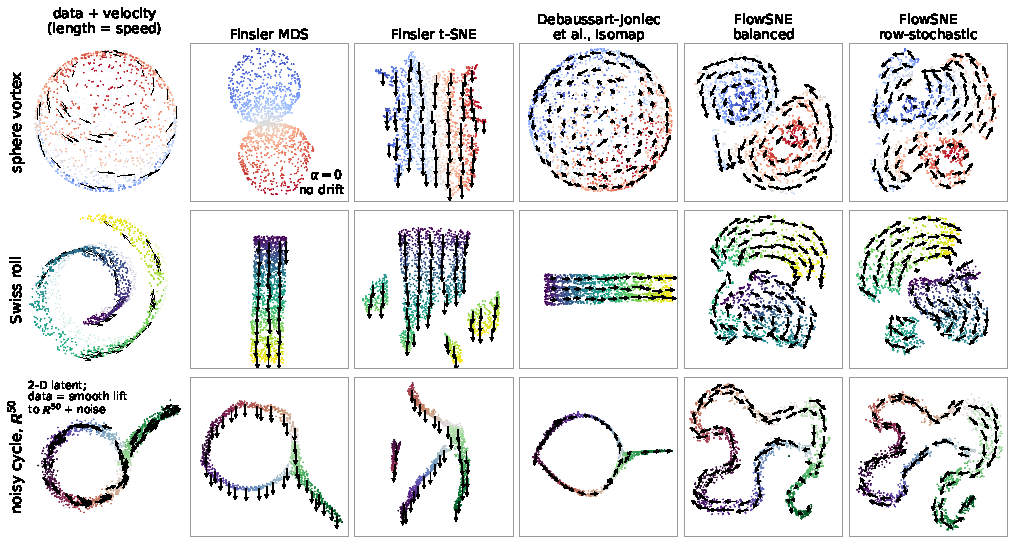
\includegraphics[width=\textwidth]{figures/table2_layouts.pdf}
  \caption{Layouts of the methods of \cref{tab:toy} (seed 0). First column:
  the data in $\mathbb{R}^3$ with the true velocity, arrow length
  proportional to speed (zero at the poles; unit speed on the Swiss roll);
  for the noisy cycle, which lives in $\R^{50}$, its 2-D latent with the
  clean velocity. Sphere coloured by height (red north, blue south), Swiss
  roll by its roll parameter, noisy cycle by phase on the ring (cyclic map)
  and by arclength on the branch (greens). Arrows: each method's drift in flow direction, averaged per
  grid cell, length relative to the panel's largest arrow (units differ
  between methods).}
  \label{fig:toy_layouts}
\end{figure*}

\paragraph{Results.}
\Cref{tab:toy,fig:toy_layouts}. A constant drift is the gradient of a linear potential, so
the two canonical-Randers baselines can only express progress along one
axis. On the Swiss roll, whose drift is a gradient, Finsler MDS on geodesic
distances unrolls the roll and is best in every column, as Isomap already is
for the layout; FlowSNE with a row-stochastic input matches its direction
($0.99$) but tears the roll into pieces. On the sphere the drift is a pure
circulation. Finsler MDS selects $\alpha=0$; Finsler t-SNE can use its drift
only by cutting the sphere along a meridian and unrolling it into a strip,
where the rotation becomes a translation (direction $0.80$), and it fits its
own objective worse than FlowSNE on the same input (cross-entropy $11.89$
against $11.62$). FlowSNE recovers the rotation ($0.95$) with the best speed
and the best neighbourhoods, directed or not; its layout keeps more
neighbours than the symmetric fit of the same affinity ($0.81$ against
$0.68$). The directed diffusion embedding is best in direction on its
Isomap layout, which keeps the fewest neighbours. On the sphere, the fitted
field has two vortex centres, on the images of the two poles
(\cref{app:toy}). The frozen-layout ablation shows what the joint fit
buys: a field fitted on the symmetric layout still finds the direction
($0.81$--$0.92$), but its speeds are wrong (Spearman $0.40$ on the sphere,
$-0.25$ on the cycle, against $0.85$ and $0.63$) and its directed
neighbourhoods stop halfway between the symmetric and the joint layout. The
direction can be painted onto a symmetric map; the speeds and the directed
neighbourhoods need the layout to move.

The noisy cycle mixes both cases in high dimension. A constant drift can
follow only one part of a ring: Finsler MDS selects $\alpha=0.2$ (direction
$0.25$), and Finsler t-SNE again cuts the ring and stacks the pieces along
its drift ($0.79$). FlowSNE recovers the mixed drift with the
row-stochastic input (direction $0.98$, speed $0.81$, kNN$_\to$ $0.61$, best
in all three) and slightly less well with the balanced one ($0.95$, $0.63$,
$0.53$), which hides the gradient parts, the pull towards the ring and the
branch. Its layouts keep as many neighbours as the symmetric fit ($0.67$
against $0.68$; the input's own 10-NN keep $0.64$ of the latent ones) and
stay connected, but draw the ring as a thin meandering line where every
direction-blind method draws a circle. This is the objective, not the
lift or the optimiser (\cref{app:fold}): a drift of norm near $\rho$
discounts forward distances, so the joint fit stretches the layout along
the flow ($1.6\times$ the symmetric ring's length for the same canvas) and
thins it, and a stretched loop in the plane meanders. Lowering $\rho$ to
$0.5$ unfolds it but destroys the speed ranking; starting the joint fit
from the symmetric layout instead of PCA reaches a lower loss and a
rounder ring with the same direction and speed. The directed diffusion
embedding is close in direction ($0.93$) but ranks speeds worse ($0.41$).


% ----------------------------------------------------------------------
\subsection{Single-cell RNA velocity}
\label{sec:exp_sc}

\paragraph{What this section tests.}
\Cref{sec:gauge} predicts that the two input affinities see different
parts of a drift: a balanced affinity sees only its cyclic part, a
row-stochastic one also its gradient part, together with the density of
the data (eq.~\ref{eq:firstorder}: it rewards a field that points at the
points with many neighbours). Three claims follow, which we test on data
where the true order of the points is known from outside the data.
(i) When the drift is mostly a gradient, the row-stochastic input is the
right one and balancing loses the signal. (ii) When the drift circulates,
the balanced input isolates the circulation, while the row-stochastic one
fits the density instead and produces a spurious field. (iii) An
embedding can lose directed information but not create it: the chain of a
map progresses at most as far as the chain of the input.

\paragraph{Data.}
Each sample is a cell, described by its gene-expression vector reduced to
30 principal components. \emph{RNA velocity} is an estimate, for every
cell, of where its expression is heading in the next hours, obtained from
the mRNA that is still being produced \citep{lamanno2018rna} or from mRNA
labelled by its age; it is a noisy vector per cell, in the same 30
coordinates. The Hodge share of \cref{sec:gauge}, computed on the 30-NN
graph, says which regime a dataset is in.
\emph{Pancreas} \citep{bastidasponce2019comprehensive} ($n=3696$,
velocity from scVelo \citep{bergen2020generalizing}): progenitor cells
mature into four hormone-producing types, a one-way process; the velocity
is $83\%$ gradient. \emph{Cell cycle} \citep{battich2020sequencing}
($n=2793$, velocity from dynamo's labelled mRNA): a human cell line in
which cells grow, copy their DNA and divide, over and over, so the
expression state moves around a loop. Two fluorescent markers, read on
each cell independently of its expression, give its position on that
loop as a number in $[0,1)$: a ground-truth phase that no method has
seen. The loop is not quite closed in the data: the cells about to divide
(the last twelfth of the loop, ``late M'') have almost no neighbours among
the cells that have just divided ($1\%$ of their 15-NN), so the loop is an
arc, and progress through its seam is the hardest test. The velocity is
$67\%$ gradient, but that part walks \emph{backwards} in phase ($-0.06$
cycle in 25 steps) and the cyclic part forward ($+0.26$): the circulating
content is exactly what balancing keeps. \emph{Gastrulation}
\citep{pijuansala2019single} ($n=30\,000$, KeOps) is the scale test; its
order is the real age of the embryo each cell was taken from.

\paragraph{Gradient regime: pancreas.}
Here the row-stochastic input is the right one (claim i): the field
FlowSNE fits agrees with the standard practice, the velocity projected
onto the map, at $0.76$ (balanced input: $0.54$), and keeps a better
layout than the directed diffusion embedding on its Isomap layout (kNN
$0.50$ against $0.29$, direction $0.69$). On gastrulation (claim iii), 25 steps of the
chain of the input affinity progress $0.37$ days further in embryo age than
a direction-blind chain, close to scVelo's own transition kernel ($0.39$);
the chain of a 10-D FlowSNE embedding keeps $0.30$ days of it, that of a
2-D map $0.13$: a map loses part of the directed information, it does not
add to it.

\begin{figure}[t]
  \centering
  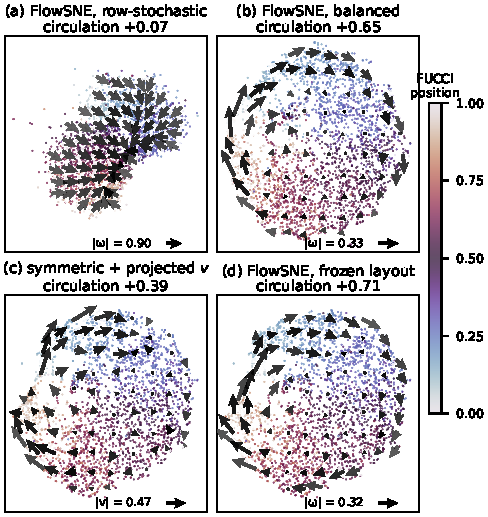
\includegraphics[width=\columnwidth]{figures/rpe1_maps.pdf}
  \caption{Cell cycle, 2-D maps, coloured by the measured phase (cyclic
  colour map, so the two ends of the scale are the same point of the loop);
  arrows: mean field per grid cell, length relative to each panel's own
  reference value (key; the row-stochastic field is saturated at $0.9$,
  the balanced ones sit near $0.1$--$0.3$). (a) Fitted jointly to the row-stochastic affinity, the field
  saturates at its bound and converges on the dense centre of the map: it
  fits the density, a gradient (eq.~\ref{eq:firstorder}), and the layout
  loses its neighbourhoods. (b) To the balanced affinity, it is
  unsaturated and circulates around the loop. (c) The symmetric layout of
  the balanced affinity with the velocity projected onto it, the standard
  practice. (d) FlowSNE with the layout frozen at (c): only the field is
  fitted, to the same balanced affinity as (b); it gives the same
  circulation as (b), on the symmetric layout.}
  \label{fig:rpe1}
\end{figure}

\begin{table}[t]
  \caption{Cell cycle, 2-D and 10-D maps (FlowSNE: 3 seeds; symmetric and
  frozen layout: seed 0). Every row uses the balanced affinity except the
  row-stochastic one. Frozen layout: the symmetric map is kept fixed and
  only the field $\omega$ is fitted, on the same loss as the joint fit.
  Circ.: does the map's field go around the loop? Net over absolute flow of
  the field around 200 loops through the 12 phase bins of the map's own
  30-NN graph ($1$: always forward, $0$: a gradient). Progress: measured
  phase gained in 10 steps of a walk that follows the field, over the same
  walk ignoring it, in cycles; late M: the same for the cells about to
  divide, which must cross the seam. kNN: 10-NN preservation, Euclidean.
  The input velocity itself, in 30 dimensions, scores $0.19$, $0.088$,
  $0.15$.}
  \label{tab:rpe1}
  \centering
  \small
  \setlength{\tabcolsep}{4pt}
  \begin{tabular}{lcccc}
    \toprule
    map / field & circ. & progress & late M & kNN \\
    \midrule
    \multicolumn{5}{l}{\emph{2-D}} \\
    symmetric + projected $v$ & 0.39 & 0.028 & 0.04 & \textbf{0.22} \\
    FlowSNE, row-stochastic & 0.07 & 0.032 & $-0.12$ & 0.09 \\
    FlowSNE, balanced & 0.68 & 0.075 & 0.08 & 0.15 \\
    FlowSNE, bal., frozen layout & \textbf{0.69} & \textbf{0.082} & \textbf{0.13} & \textbf{0.22} \\
    \midrule
    \multicolumn{5}{l}{\emph{10-D}} \\
    symmetric + projected $v$ & \textbf{0.35} & 0.048 & 0.05 & \textbf{0.30} \\
    FlowSNE, row-stochastic & 0.13 & 0.166$^\ast$ & $-0.08$ & 0.27 \\
    FlowSNE, balanced & 0.31 & 0.059 & \textbf{0.15} & 0.28 \\
    \bottomrule
  \end{tabular}
  \par\smallskip\raggedright\footnotesize
  $^\ast$A density artefact: the field points at the dense regions, which
  happen to lie forward in phase for most cells and backward for the
  late-M ones (see text).
\end{table}

\paragraph{Circulating regime: the cell cycle.}
\Cref{fig:rpe1,tab:rpe1}. The row-stochastic input fails as predicted
(claim ii). Its fitted field is $98\%$ gradient on the map's own graph and
saturates at its bound (median $|\omega|=0.90$; with the bound lowered to
$\rho=0.5$ it saturates at $0.47$, still $98\%$ gradient): it points at
the dense regions, and the walk that follows it sends the cells about to
divide backwards ($-0.12$); the joint fit also wrecks the layout (kNN
$0.09$). The balanced input isolates the circulation. Its field is $77\%$
cyclic and goes around the loop with circulation $0.68$, against $0.39$
for the velocity projected onto the same symmetric layout and $0.19$ for
the velocity itself in 30 dimensions: balancing has extracted the
rotational part of a velocity that was two-thirds gradient. A walk on the
fitted field gains as much phase as a walk on the input velocity ($0.08$
against $0.09$ cycle in 10 steps), 2.7 times the projected arrows, and
the cells about to divide move forward, across the seam. The joint 2-D fit
pays for this in neighbourhoods (kNN $0.15$ against $0.22$): in two
dimensions the directed structure lives in the field, not in the layout.
Fitting the field alone on the frozen symmetric layout gives the same
field at no cost (last 2-D row), which is the recipe we recommend for
maps. In 10 dimensions (3 seeds) the joint fit keeps the neighbourhoods
(kNN $0.282 \pm 0.001$ against $0.304$) and its own chain progresses
$0.072 \pm 0.001$ cycle in 10 steps, against $0.048$ for the projection
($0.127$ against $0.062$ across the seam); with dynamo's smoothed
velocity, $0.229 \pm 0.004$ against $0.125$, as far as the chain of the
input itself ($0.236$), the bound of claim (iii). There the field
saturates again (median $|\omega| = 0.88$) and its circulation is no
better than the projection's ($0.31$ against $0.35$): with room for the
directed structure in the layout, the gain is in the chain, not in the
field. The row-stochastic 10-D field walks further overall ($0.17$) but
is the density artefact again: saturated ($|\omega| = 0.93$), circulation
$0.13$, late-M cells backward ($-0.08$).
\todo[inline]{dynamo's smoothed velocity as a second column of
Table~\ref{tab:rpe1} if space allows.}

% ----------------------------------------------------------------------
\subsection{Transformer residual streams}
\label{sec:exp_transformer}

\begin{figure}[t]
  \centering
  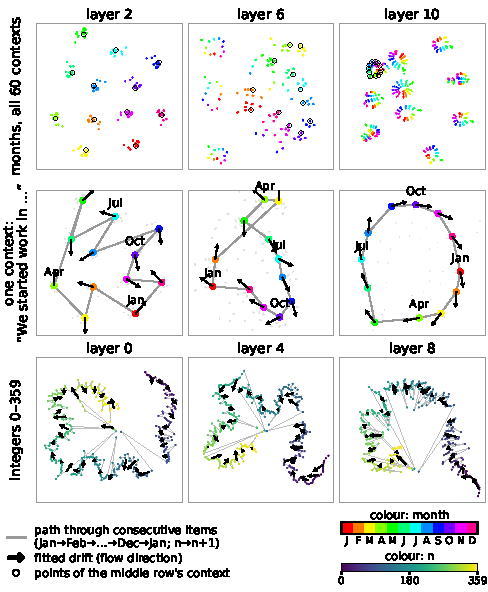
\includegraphics[width=\columnwidth]{figures/transformer_concepts.pdf}
  \caption{GPT-2 small, FlowSNE with a row-stochastic input; the input drift
  of each point is its successor in the same context. Arrows: fitted drift
  in flow direction. Grey line: the path through consecutive items
  (January$\to\dots\to$December$\to$January, $n\to n+1$).
  \emph{Top:} the 12 months at the end of 60 sentence contexts, at layers 2,
  6 and 10; the context of the middle row is circled. \emph{Middle:} that
  context alone: its months are scattered over the month clusters at layer
  2 and form a ring in calendar order by layer 10, which the drift turns
  around. \emph{Bottom:} integers 0--359 (mean over 10 contexts): one line
  with a wiggle per decade, the drift running along it; the straight grey
  segments are the jumps $10k{-}1\to 10k$ into the cluster of multiples of
  10 at the centre.}
  \label{fig:transformer}
\end{figure}

\todo[inline]{Section 6.3 text: setting (GPT-2 small, concept token,
successor drift), probe: last digit decodable but categorical, no helix in GPT-2 small (last-digit centroids equidistant); 3-D maps form no coil, rings already in
symmetric t-SNE (winding 0.88--1.00 vs 0.25--0.55 shuffled), FlowSNE
orients them (succ.\ cos 0.61--0.84, turning agrees 83--100\%), Finsler
t-SNE picks $\alpha=0$; numbers = gradient regime; residual-update drift is
${\sim}90\%$ constant (gauge). One seed so far.}


% ======================================================================
\section{Conclusion and discussion}
\label{sec:conclusion}

\todo[inline]{Section 7, to be written.}


\bibliography{references}
\bibliographystyle{icml2026}

\newpage
\appendix
\onecolumn
% ======================================================================
\section{Computing Randers distances}
\label{app:randers}

\paragraph{Low dimension: eikonal solvers.}
For a fixed source $x_0$, $u=\dF(x_0\to\cdot)$ is the viscosity solution
of the eikonal equation $F^*_x(\nabla u)=1$, $u(x_0)=0$, with $F^*_x$ the
dual norm, again of Randers type by Zermelo's navigation
\citep{bao2000introduction}. Ordered-upwind and adaptive-stencil fast
marching handle asymmetric metrics on a grid
\citep{sethian2003ordered,mirebeau2014efficient}, at $O(N\log N)$ per
source on $N$ nodes and $n$ sources for a full cost matrix. This is
practical in $d=2$ or $3$ only.

\paragraph{High dimension.}
A grid with $m$ nodes per axis has $m^d$ nodes. Graph substitutes run
Dijkstra's algorithm on a directed kNN graph with local Randers edge
lengths, as Isomap does for Euclidean geodesics
\citep{tenenbaum2000global}; heat-kernel proxies replace the infimum by a
small-time limit of a diffusion. Both converge only as the samples
densify around the optimal paths, and both are biased towards dense
regions.

\paragraph{The drift is only sampled.}
The infimum ranges over paths through regions where $\omega$ is not
measured, so its value depends on how $\omega$ is extended between
samples. That is a modelling choice the data do not support.

\paragraph{Proof of \cref{prop:approx}.}
\emph{(1)} Let $g(t)=\omega(x+t\Delta)^\top\Delta$ with $\Delta=y-x$, so
$\ell(x,y)=r+\int_0^1g$. The frozen form replaces $\int_0^1g$ by $g(0)$,
with error at most $\tfrac12\sup|g'|\le\tfrac12L_1r^2$; the averaged form
by $\tfrac12(g(0)+g(1))$, the trapezoid rule, with error at most
$\tfrac1{12}\sup|g''|\le\tfrac1{12}L_2r^3$.
\emph{(2)} \tbd{Make rigorous.} $\ell\ge\dF$ since the segment is one of
the paths. Let $\gamma$ be any path from $x$ to $y$ with Euclidean length
$r+e$ and maximal distance $h$ to the segment. Its Randers length minus
$\ell$ is $e+\oint_\sigma\omega\cdot dx$, where $\sigma$ is the closed
loop $\gamma$ followed by the reversed segment. By Stokes' theorem the
loop integral is bounded by $\tfrac12L_c$ times the area of a surface
spanning $\sigma$, at most $(r+e)h$ for the cone from $x$. A path that
deviates by $h$ has $e\ge c_0\min(h,h^2/r)$. Hence the Randers length of
$\gamma$ is at least $\ell+c_0\min(h,h^2/r)-\tfrac12L_c(r+e)h$; for
$L_cr\le c'$ the minimum over $h$ and $e$ is at least $\ell-cL_c^2r^3$.
\emph{(3)} For $\omega=\nabla\phi$ the drift integral along any path is
$\phi(y)-\phi(x)$, and the Euclidean length is minimised by the segment.

\paragraph{Numerical check.}
\tbd{Table: Study A (experiments/ot), relative errors of the two forms on
gradient drifts in $D=50$ against the exact distance, as a function of
$\|\omega\|$ and neighbourhood size.}

% ======================================================================
\section{Proofs for \cref{sec:gauge}}
\label{app:proofs}

\begin{lemma}[Structure of $\Sep$]
  $\Sep=\{(s_i+s_j)_{ij}:s\in\R^n\}\oplus\Grad$ and $\Sep\cap\Asym=\Grad$.
\end{lemma}
\begin{proof}
  Write $f_i+g_j=(s_i+s_j)+(\psi_j-\psi_i)$ with $s=\tfrac12(f+g)$ and
  $\psi=\tfrac12(g-f)$; the first term is symmetric and the second
  antisymmetric, so the sum is direct. If $f_i+g_j$ is antisymmetric, its
  diagonal gives $g=-f$, hence $f_i+g_j=f_i-f_j\in\Grad$.
\end{proof}

\begin{proof}[Proof of \cref{thm:identifiability}]
  The kernel is entrywise positive, so the scaling exists and the coupling
  is unique \citep{sinkhorn1967concerning}. If $C'_{ij}=C_{ij}+f_i+g_j$,
  then $e^{-C'/\eps}=\diag(e^{-f/\eps})\,e^{-C/\eps}\diag(e^{-g/\eps})$;
  the diagonal factors are absorbed into the scalings, and uniqueness gives
  the same coupling. Conversely, if both couplings equal $P$, then
  $\log P_{ij}=\log u_i+\log v_j-C_{ij}/\eps=\log u'_i+\log v'_j-C'_{ij}/\eps$,
  so $C-C'\in\Sep$. The second statement follows from the lemma.
\end{proof}

\paragraph{Cyclic part.}
Adding $G\in\Grad$ to $A$ shifts the minimiser in the definition of
$\cyc_W$ by $G$, so $\cyc_W(A+G)=\cyc_W(A)$; conversely, equal cyclic parts
force $A-A'$ to be a difference of minimisers, a gradient. The normal
equations give $\sum_jW_{ij}\cyc_W(A)_{ij}=0$ for every $i$.

\paragraph{Net flow.}
If $P\1=P^\top\1=a$, then $\sum_{ij}P_{ij}(f_j-f_i)=\sum_ja_jf_j-\sum_ia_if_i=0$.
Taking $f=\1_k$ gives $((P-P^\top)\1)_k=0$. The chain $\diag(a)^{-1}P$ has
stationary law $a$, and so do its powers.

\paragraph{An optimal transport reading.}
On couplings with marginals $a,b$,
$\sum_{ij}P_{ij}(C_{ij}+f_i+g_j)=\langle P,C\rangle+\langle a,f\rangle+\langle b,g\rangle$:
a separable change of cost shifts every transport cost by the same
constant and leaves optimal plans unchanged, with or without entropy.
For an exact gradient drift, unregularised OT under the Randers cost
therefore has the optimal plans of the Euclidean $W_1$ problem. The
converse of \cref{thm:identifiability} needs entropy: an unregularised
plan constrains the cost only through cycle sums.

% ======================================================================
\section{Hodge decompositions}
\label{app:hodge}

\begin{figure}[h]
  \centering
  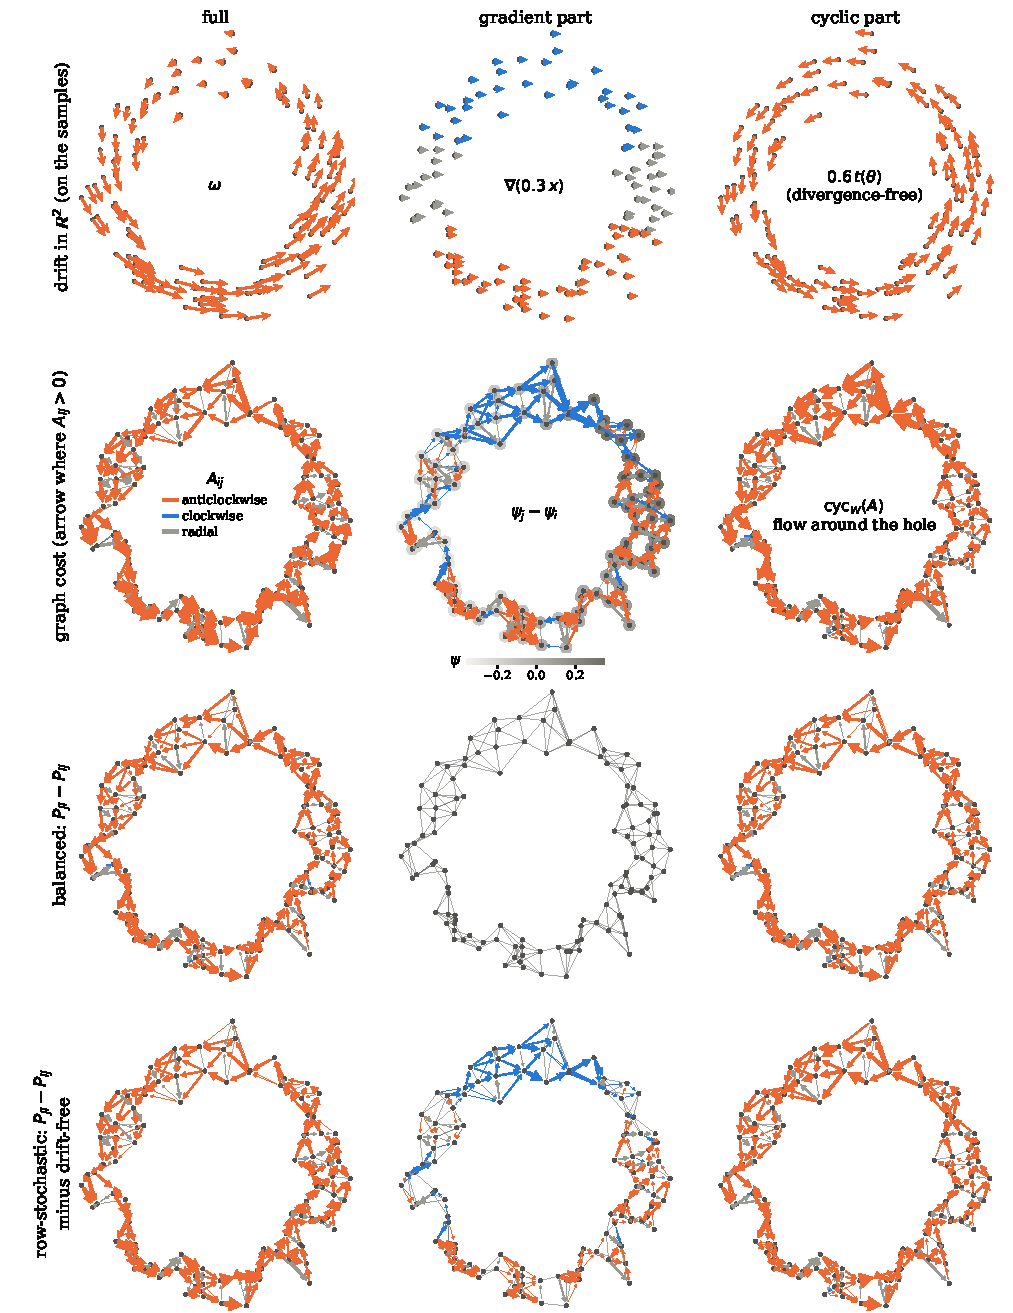
\includegraphics[width=0.7\textwidth]{figures/hodge_ring.pdf}
  \caption{Weighted Hodge decomposition on a ring (120 points, symmetrised
  5-NN graph, linear cost, global bandwidth). The drift is
  $\omega=0.6\,t(\theta)+0.3\,e_x$, a rotation, which is harmonic on the
  ring, plus a uniform drift, an exact gradient. Columns: full, gradient
  part, cyclic part. Rows: the drift in $\R^2$; the graph cost
  $A_{ij}$, arrow $i\to j$ where $A_{ij}>0$, width $\propto|A_{ij}|$,
  coloured by orientation around the ring; the balanced affinity's net
  transport $P_{ji}-P_{ij}$, which carries no gradient part; the
  row-stochastic one's, minus that of the drift-free affinity, which
  carries both.}
  \label{fig:hodge_full}
\end{figure}

\paragraph{Real velocity fields.}
\label{app:hodge_data}
\tbd{Table: gastrulation ($n=30\,000$, 30-NN graph in 30-PC space):
gradient share 0.75--0.83 (null 0.31--0.33), and a walk on the cyclic part
alone gains no days; RPE1-FUCCI ($n=2793$): gradient share 0.67 for the
direct velocity, but its gradient part walks backwards around the cycle
($-0.06$ cycle after 25 steps) while the curl part advances ($+0.26$).}

% ======================================================================
\section{What the output loss rewards}
\label{app:output}

\tbd{Test 1 of experiments/theory/output\_kernel.py: first-order loss
sensitivity at the symmetric fit to gradient vs rotated perturbations of
the output drift, Student and Laplace kernels, pancreas and RPE1, balanced
and row-stochastic inputs, $q=2$ and $q=1$. Exact cancellation for the
Laplace kernel with an exact potential cost ($10^{-14}$).}

% ======================================================================
\section{Implementation details}
\label{app:implementation}

Both Randers affinities accept any backend of TorchDR.

\paragraph{Costs from matrix products.}
The drift term of \eqref{eq:averaged} rearranges to
\[
  A_{ij}=\tfrac12\big[(\Omega X^\top)_{ij}-(X\Omega^\top)_{ij}+s_j-s_i\big],
  \qquad s_i=\omega_i^\top x_i ,
\]
with $\Omega$ the matrix of drifts, so the cost needs $(n,n)$ products and
never the $(n,n,D)$ tensor of differences: at $n=2000$, $D=100$, this is
$100\times$ faster (0.07~s against 7.5~s) and avoids a 3.2~GB tensor.

\paragraph{Linear memory with KeOps.}
With KeOps \citep{charlier2021keops}, the output cost \eqref{eq:Q} is a
symbolic lazy tensor: the normaliser $\sum_{k\neq l}(1+\dav_\theta^2)^{-1}$
and its gradients are reduced on the fly, in $O(n)$ memory. The input
affinity is made sparse by keeping, in each row, the $k=5\mathcal{P}$
nearest points under the \emph{directed} cost, found by a KeOps
$\arg\min_k$; the loss \eqref{eq:loss} then splits into an attraction on
the $nk$ kept entries and the lazy normaliser. Dense and KeOps paths agree
to $10^{-15}$ in float64 on losses and gradients.

\paragraph{Sinkhorn.}
A per-row perplexity bandwidth makes the balanced kernel badly
conditioned: thousands of iterations are needed to reach marginal errors
below $10^{-4}$. We run Sinkhorn in the log domain, in float32 if needed,
with early stopping on the marginal error. On kNN-sparse inputs we balance
the kNN graph with its reverse edges; this is a local variant of balancing
rather than an approximation of the dense one, so we use row-stochastic
affinities at scale.

\begin{table}[h]
  \caption{Time per optimisation step (loss, backward, Adam step) and peak
  memory, RTX 2080 Ti, float32, $k=250$. Dense runs are skipped when they
  would exceed the GPU's memory.}
  \label{tab:scaling}
  \centering
  \small
  \setlength{\tabcolsep}{4pt}
  \begin{tabular}{rcccc}
    \toprule
    $n$ & input aff. & KeOps step & memory & dense step \\
    \midrule
    $10^4$ & 1.7~s & 0.020~s & 0.26~GB & 0.097~s \\
    $2\cdot10^4$ & 2.4~s & 0.034~s & 0.49~GB & -- \\
    $5\cdot10^4$ & 8.1~s & 0.112~s & 1.21~GB & -- \\
    $10^5$ & 19.9~s & 0.359~s & 1.73~GB & -- \\
    \bottomrule
  \end{tabular}
\end{table}

\paragraph{Performance.}
\Cref{tab:scaling} shows the scaling: memory grows linearly, and a
3000-step fit of $10^5$ points takes about 18 minutes on a consumer GPU.
Quality holds at scale: on a synthetic vortex with $n=5\cdot10^4$, the
fitted speed correlates at $0.94$ with the true one (against $0.89$ at
$n=1500$), provided the perplexity grows as $\sqrt n$; capping it at $50$
halves the cost but drops the correlation to $0.82$.

% ======================================================================
\section{Architectures that did not help}
\label{app:architecture}

\tbd{Short summary with numbers from experiments/toy/stream\_sphere.py:
a $64\times2$ MLP matches the $32\times1$ one; random Fourier features
improve direction slightly at the same loss; a divergence-free drift
$\omega=J\nabla h$ loses 40--60\% of the loss gain and folds the layout,
because a push-forward under a map that does not preserve area is not
divergence-free; an exact potential drift ($\omega=\nabla h$) gives
slightly worse layouts than the symmetric fit.}

% ======================================================================
\section{Synthetic flows: details}
\label{app:toy}

\tbd{Protocol (Adam learning rates, iterations, $\rho$, perplexity),
vortex-centre analysis of the sphere fits (experiments/toy/stream\_sphere.py
poles), and the figure of all layouts.}

\paragraph{Why the ring folds.}
\label{app:fold}
On the noisy cycle every direction-blind layout (symmetric t-SNE of the
same affinity, Finsler MDS, Isomap) draws the ring as a convex loop, and
every FlowSNE joint fit as a thin meandering line (\cref{fig:toy_layouts}).
\Cref{tab:fold} scores the ring's shape by the convexity of the polygon
through its 24 phase-bin centroids (area over convex-hull area) and by its
total turning in units of $2\pi$; a convex loop scores $1$ on both. The
optimiser schedule is not the cause: early exaggeration, a cosine learning
rate, a ten times smaller rate for the flow and a warm-up leave the shape
unchanged. Nor is the lift: with a linear lift to $\R^{50}$ (no sine
features) the ring folds the same. The cause is the objective. A drift of
norm $|\omega|$ makes a forward step of length $r$ cost $(1-|\omega|)r$,
so to reproduce the input's affinity decay the joint fit stretches the
layout along the flow and thins it: the ring's perimeter relative to the
layout's r.m.s.\ radius is $5.2$--$5.4$ for the symmetric layouts
($2\pi$ for a circle), $8.3$--$8.5$ for the joint fits, and its
transverse width halves. A stretched loop in the plane meanders. Lowering
the bound to $\rho=0.5$ halves the stretch ($6.4$) and nearly unfolds the
ring, but the field can no longer rank speeds. A warm start from the
symmetric layout, instead of PCA, reaches a lower loss than the PCA start
on every seed, with a rounder ring and the same direction and speed: the
PCA-started fit settles in a more folded local minimum. The exact circle
with the best field fitted on it has the highest loss of all
($11.55$): the loss genuinely prefers some bending.

\begin{table}[h]
  \caption{Noisy cycle, seed 0 (warm start: 3 seeds), balanced / row-stochastic input.
  Direction, speed and loss as in \cref{tab:toy}; conv.\ and turn: ring shape (1 = convex loop).}
  \label{tab:fold}
  \centering
  \small
  \setlength{\tabcolsep}{3pt}
  \begin{tabular}{lccccc}
    \toprule
    joint fit & dir. & speed & loss & conv. & turn \\
    \midrule
    symmetric layout (no drift) & -- & -- & -- & 1.00 / 1.00 & 1.04 / 1.01 \\
    PCA start (\cref{tab:toy}) & 0.95 / 0.98 & 0.53 / 0.75 & 11.41 / 11.43 & 0.67 / 0.66 & 2.7 / 2.6 \\
    \quad + exagg., cosine, flow lr, warm-up & 0.95--0.96 / 0.97--0.98 & -- & 11.41--11.53 & 0.66--0.70 / 0.62--0.70 & 2.6--2.8 \\
    \quad with $\rho=0.5$ & 0.94 / 0.97 & $-0.20$ / 0.37 & 11.51 / 11.56 & 0.88 / 0.89 & 1.6 / 1.6 \\
    \quad linear lift, no sines & 0.83 / 0.98 & 0.42 / 0.63 & 11.38 / 11.42 & 0.67 / 0.62 & 2.4 / 2.6 \\
    warm start from symmetric layout & 0.96 / 0.98 & 0.62 / 0.78 & 11.33 / 11.36 & 0.76 / 0.83 & 2.3 / 2.2 \\
    \quad with $\rho=0.7$ & 0.95 / 0.97 & 0.47 / 0.49 & 11.39 / 11.44 & 0.90 / 0.94 & 1.5 / 1.5 \\
    field fitted on the frozen circle & 0.93 / 0.88 & $-0.25$ / $-0.06$ & 11.55 / -- & 1.00 & 1.0 \\
    \bottomrule
  \end{tabular}
\end{table}



\end{document}
